\chapter{DESAIN DAN IMPLEMENTASI}
\label{chap:desainimplementasi}

% Ubah bagian-bagian berikut dengan isi dari desain dan implementasi

Penelitian ini dilaksanakan sesuai dengan sistem berikut dengan implementasinya. Desain sistem merupakan konsep dari pembuatan dan perancangan infrastruktur dan kemudian diwujud kan dalam bentuk blok-blok alur yang harus dikerjakan. Pada bagian implementasi merupakan pelaksanaan teknis untuk setiap blok pada desain sistem.

\section{Deskripsi Sistem}
\label{sec:deskripsisistem}

Sistem pada tugas akhir ini merupakan implementasi dari salah satu disiplin ilmu \textit{Deep Learning} dan pengolahan citra yang berfungsi untuk mendeteksi adanya pejalan kaki yang berada di pinggir jalan, trotoar dan jalur penyebrangan. Selain pejalan kaki, deteksi juga dilakukan pada jalur penyebrangan atau \textit{zebracross} dengan tujuan untuk memberi informasi bahwa disekitar area tersebut terdapat banyak aktivitas pejalan kaki yang menyebrang jalan. Blok diagram metodologi sistem yang digunakan pada penelitian ini dapat dilihat pada Gambar \ref{fig:blok-diagram}.

\begin{figure}[ht]
	\centering
	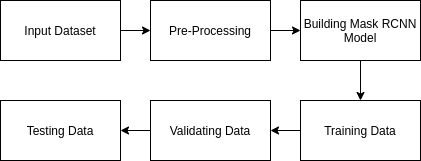
\includegraphics[scale=0.5]{gambar/blok-diagram.png}
	\caption{Blok Diagram Metodologi}
	\label{fig:blok-diagram}
\end{figure}  

\section{Pengumpulan \textit{Dataset} Gambar}
\label{sec:pengumpulandatagambar} 

Pada tugas akhir ini, \textit{dataset} yang digunakan didapatkan dengan beberapa cara, antara lain:
	\begin{enumerate}
		\item \textit{Caltech Pedestrian Database}, merupakan kumpulan gambar yang diambil dari sudut pandang pengendara mobil di California Amerika Serikat dengan ukuran 640 x 480 pixel. Terdapat sekitar 250.000 gambar dengan 350.000 \textit{bounding boxes} dan sekitar 2.300 pejalan kaki dengan kriteria unik diberi tanda. Namun, pada \textit{dataset} ini hanya pejalan kaki saja yang diberi label, sehingga perlu dilakukan proses pelabelan ulang sesuai kelas yang diinginkan. Tidak semua gambar pada \textit{dataset} ini diambil untuk digunakan, gambar yang mempunyai objek berupa pejalan kaki dan \textit{zebracross} saja yang akan digunakan. Gambar \ref{fig:caltech} merupakan contoh dari gambar yang terdapat pada \textit{Caltech Pedestrian Database}.
		\begin{figure}[ht]
			\centering
			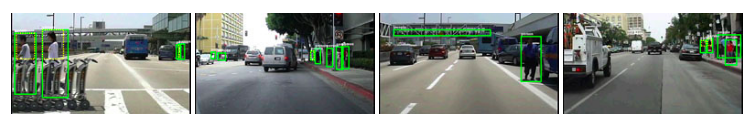
\includegraphics[scale=0.35]{gambar/caltech.png}
			\caption{Contoh Gambar dari Caltech Pedestrian Database}
			\label{fig:caltech}
		\end{figure} 
		
		\item Tangkapan layar dari beberapa video \textit{online Youtube}. Pada cara ini, penulis mencari video yang berada pada salah satu \textit{website video streaming} yaitu Youtube dengan persyaratan video diambil dari sudut pandang pengendara mobil yang berkendara pada jalan raya dengan ukuran gambar 1360x768 px. Pada \textit{frame-frame} tertentu dilakukan \textit{screenshot} dan disimpan untuk selanjutnya dilakukan proses pemberian label pada objek-objek yang diinginkan seperti pada Gambar \ref{fig:youtube-dataset}. 
		
		\begin{figure}[ht]
			\centering
			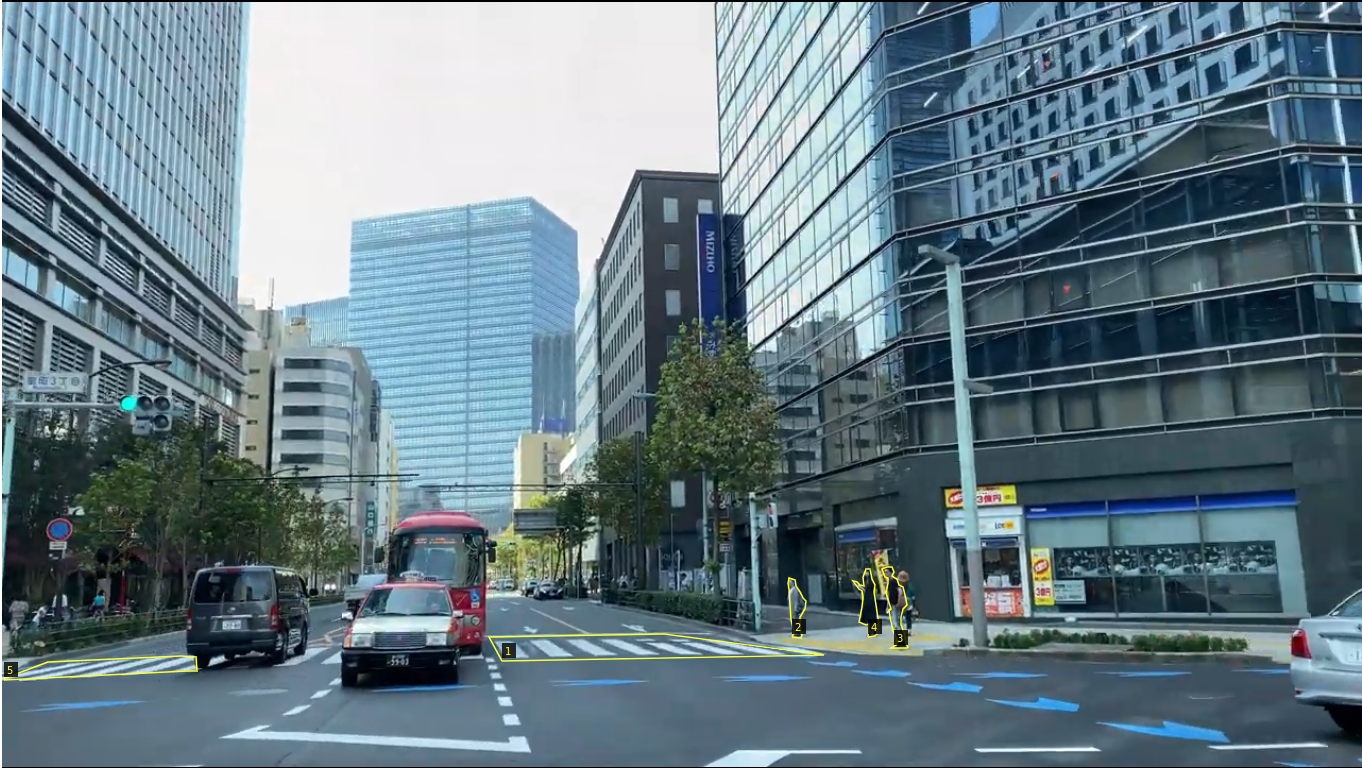
\includegraphics[scale=0.15]{gambar/youtube-dataset.png}
			\caption{Contoh Pembuatan \textit{dataset} dari \textit{Screenshot Youtube}}
			\label{fig:youtube-dataset}
		\end{figure}
		
		\item Pengambilan gambar secara mandiri menggunakan kamera \textit{smartphone} yang diambil dari sudut pandang pengendara motor dengan ukuran gambar yang diambil sebesar 1280x720 px. Pengambilan gambra dilakukan di jalan-jalan Surabaya. Setelah dilakukan pengambilan gambar, proses selanjutnya adalah pemberian label pada objek-objek yang ingin dideteksi.
	\end{enumerate}

\section{Pemisahan Data}
\label{sec:pemisahandata}

Dalam \textit{machine learning} pemisahan data ke beberapa \textit{subset} merupakan suatu hal yang sangat penting. Hal ini dikarenakan setiap \textit{subset} memiliki fungsi masing-masing. Gambar \ref{fig:data-splitting} merupakan rasio pembagian data ke masing-masing subset.

\begin{figure}[ht]
	\centering
	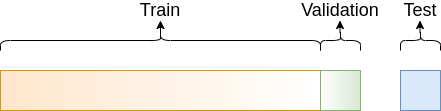
\includegraphics[scale=0.5]{gambar/data-splitting.png}
	\caption{Visualisasi Pembagian Data}
	\label{fig:data-splitting}
\end{figure}

\begin{enumerate}
	\item \textit{Training Sets}\\
	\textit{Training Sets} merupakan sampel data yang digunakan untuk melatih model yang sudah kita buat, dalam bidang \textit{Neural Network} bisa disebut juga bobot dan bias. Model yang sudah kita buat mempelajari pola masukan dan keluaran dari data ini. 
	
	\item \textit{Validation Sets}\\
	\textit{Validation Sets} merupakan sampel data yang digunakan untuk mengevaluasi model yang sudah dilatih menggunakan \textit{training sets}. Selain itu, data ini digunakan untuk memperbarui dan menyempurnakan hyperparameter dari model ke tingkat yang lebih tinggi.
	
	\item\textit{Test Sets}\\
	\textit{Test Sets} merupakan sampel data yang digunakan untuk mengevaluasi model akhir setelah melalui proses \textit{training dan validation}. Apabila pengujian model pada data ini sudah sesuai dengan yang diinginkan, maka proses \textit{learning} sudah selesai. Namun apabila pengujian tidak sesuai dengan yang diharapkan maka diperlukan pengaturan ulang mulai dari proses \textit{training}. 
\end{enumerate}

\section{\textit{Pre-Processing}}
\label{sec:preprocessing}

Pada tahap ini, gambar-gambar dari \textit{dataset} akan mengalami proses penyesuaian sebelum masuk ke proses \textit{data training}. Setiap gambar yang akan dijadikan bahan pembelajarnan model harus memiliki dimensi dan kedalaman yang sama. Tujuan dari \textit{pre processing} adalah perbaikan data gambar dengan menekan distorsi yang tidak diinginkan atau meningkatkan beberapa fitur gambar yang relevan untuk pemrosesan lebih lanjut. Gambar \ref{fig:preprocessing} merupakan tahapan dari \textit{pre-processing} gambar \textit{dataset} yang dilakukan.

\begin{figure}[ht]
	\centering
	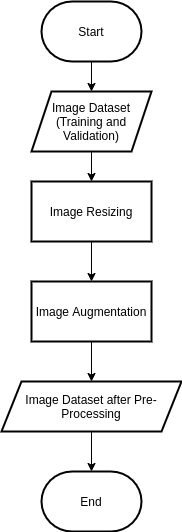
\includegraphics[scale=0.5]{gambar/flowchart-preprocessing.png}
	\caption{Diagram Alir \textit{Pre Processing}}
	\label{fig:preprocessing}
\end{figure}

Berikut merupakan penjelasan mengenai tahapan \textit{pre-processing} yang dilakukan pada tugas akhir kali ini:
\begin{enumerate}
	\item \textit{Image resizing}\\
		Langkah awal dari proses \textit{pre-processing} adalah memastikan semua gambar dalam \textit{dataset} kita memiliki ukuran yang sama. Selain itu, sama seperti sebagian besar model dari \textit{neural network} lainnya, metode yang dilakukan penulis juga mengasumsikan gambar \textit{input} berbentuk persegi. Jadi diperlukan pemeriksaan gambar di awal, apakah gambar sudah berbentuk persegi atau belum. Berbeda dari metode \textit{image resizing} pada model \textit{neural network} lainnya yang menggunakan teknik \textit{cropping} untuk membuat aspek rasio gambar input menjadi persegi, penulis menggunakan metode yang sudah terdapat pada \textit{Mask R-CNN}.
		
		Ukuran gambar yang penulis pilih pada tugas akhir kali ini adalah 512x512 pixel. Pemilihan ukuran gambar ini dilakukan untuk mengurangi beban dan waktu saat \textit{training data}. Apabila terdapat gambar pada \textit{dataset} dengan ukuran baik panjang maupun lebar lebih dari 512 pixel. maka gambar akan di \textit{down scaling} sampai ukuran 512 pixel. Sebaliknya, apabila ada gambar pada \textit{dataset} dengan ukuran lebih kecil dari 512 pixel maka akan dilakukan \textit{up scaling} sampai gambar berukuran 512 pixel. Aspek rasio gambar yang sudah melalui proses \textit{scaling} tetap dipertahankan, namun diperlukan penambahan \textit{zero padding} untuk membuat gambar \textit{input} menjadi persegi seperti yang diinginkan.
		
		\begin{figure}[ht]
			\centering
			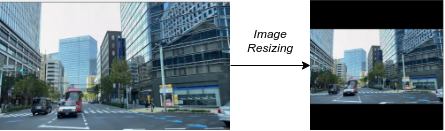
\includegraphics[scale=0.7]{gambar/image-resizing.png}
			\caption{Contoh \textit{Image Resizing}}
			\label{fig:image-resizing}
		\end{figure}
		
		Gambar \ref{fig:image-resizing} merupakan salah satu contoh \textit{image resizing} yang dilakukan. Gambar \textit{input} (gambar sebelah kiri) mempunyai ukuran 768x1360 dengan kedalaman 3 atau mempunyai format warna RGB. Setelah mengalami \textit{image resizing} (gambar sebelah kanan) ukuran gambar menjadi 290x512. Namun untuk membuat gambar memiliki aspek rasio 1:1 (berbetuk persegi) maka diperlukan penambahan \textit{zero padding} pada bagian atas gambar sebesar 111 pixel dan pada bagian bawah gambar sebesar 111 pixel. Dengan penambahn \textit{padding} seperti itu membuat gambar \textit{input} berbentuk persegi namun tidak mengurangi informasi gambar. 
		   
	\item \textit{Image Augmentation}\\
	Langkah selanjutnya pada \textit{pre-processing} adalah \textit{image augmentaion}. Proses augmentasi yang dilakukan pada tugas akhir ini adalah rotasi dan transformasi. Tujuan dari penggunanaan \textit{image augmentation} adalah untuk mengekspos \textit{neural network} ke berbagai variasi, agar dapat mengenali fitur yang akan dilakukan pada proses \textit{training}. Hal tersebut akan sangat membantu \textit{neural network} untuk mengenali variasi yang tidak terdapat pada dataset. Seperti yang terdapat pada Gambar \ref{fig:image-augmentation}, tanpa ada augmentasi maka \textit{neural network} hanya mengenali satu kondisi saja. Jika memakai augmentasi gambar seperti transformasi, maka setidaknya \textit{neural network} akan dapat mengenali 2 kondisi. Semakin banyak augmentasi yang digunakan semakin banyak pula kondisi yang bisa dikenali oleh \textit{neural network}. Namun semakin banyak kondisi yang dikenali, semakin lama dan berat proses \textit{training data} yang dilakukan. 
	
	\begin{figure}[ht]
		\centering
		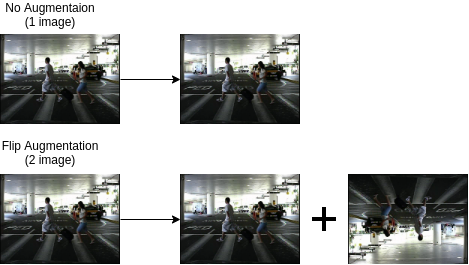
\includegraphics[scale=0.5]{gambar/image-augmentation.png}
		\caption{Contoh \textit{Image Augmentation}}
		\label{fig:image-augmentation}
	\end{figure}
	  
\end{enumerate}

\section{Membangun Model Mask R-CNN
\label{sec:membangunmodelmaskrcnn}}

\section{\textit{Training Data}
	\label{sec:trainingdata}}

\section{\textit{Validating Data}
	\label{sec:validatingdata}}

\section{\textit{Testing Data}
	\label{sec:testingdata}}

\section{Implementasi Alat
\label{sec:implementasi alat}}

Alat diimplementasikan dengan \lipsum[1]

% Contoh pembuatan potongan kode
\begin{lstlisting}[
  language=C++,
  caption={Program halo dunia.},
  label={lst:halodunia}
]
#include <iostream>

int main() {
    std::cout << "Halo Dunia!";
    return 0;
}
\end{lstlisting}

\lipsum[2-3]

% Contoh input potongan kode dari file
\lstinputlisting[
  language=Python,
  caption={Program perhitungan bilangan prima.},
  label={lst:bilanganprima}
]{program/bilangan-prima.py}

\lipsum[4]
